% (find-LATEX "2023-1-ES-P2.tex")
% (defun c () (interactive) (find-LATEXsh "lualatex -record 2023-1-ES-P2.tex" :end))
% (defun C () (interactive) (find-LATEXsh "lualatex 2023-1-ES-P2.tex" "Success!!!"))
% (defun D () (interactive) (find-pdf-page      "~/LATEX/2023-1-ES-P2.pdf"))
% (defun d () (interactive) (find-pdftools-page "~/LATEX/2023-1-ES-P2.pdf"))
% (defun e () (interactive) (find-LATEX "2023-1-ES-P2.tex"))
% (defun o () (interactive) (find-LATEX "2023-1-ES-P1.tex"))
% (defun u () (interactive) (find-latex-upload-links "2023-1-ES-P2"))
% (defun v () (interactive) (find-2a '(e) '(d)))
% (defun d0 () (interactive) (find-ebuffer "2023-1-ES-P2.pdf"))
% (defun cv () (interactive) (C) (ee-kill-this-buffer) (v) (g))
%          (code-eec-LATEX "2023-1-ES-P2")
% (find-pdf-page   "~/LATEX/2023-1-ES-P2.pdf")
% (find-sh0 "cp -v  ~/LATEX/2023-1-ES-P2.pdf /tmp/")
% (find-sh0 "cp -v  ~/LATEX/2023-1-ES-P2.pdf /tmp/pen/")
%     (find-xournalpp "/tmp/2023-1-ES-P2.pdf")
%   file:///home/edrx/LATEX/2023-1-ES-P2.pdf
%               file:///tmp/2023-1-ES-P2.pdf
%           file:///tmp/pen/2023-1-ES-P2.pdf
%  http://anggtwu.net/LATEX/2023-1-ES-P2.pdf
% (find-LATEX "2019.mk")
% (find-Deps1-links "Caepro5 Piecewise1")
% (find-Deps1-cps   "Caepro5 Piecewise1")
% (find-Deps1-anggs "Caepro5 Piecewise1")
% (find-MM-aula-links "2023-1-ES-P2" "ES" "esm231p2" "esp2")

% «.defs»			(to "defs")
% «.defs-T-and-B»		(to "defs-T-and-B")
% «.defs-caepro»		(to "defs-caepro")
% «.defs-pict2e»		(to "defs-pict2e")
% «.defs-dots»			(to "defs-dots")
% «.title»			(to "title")
% «.questao-1»			(to "questao-1")
% «.questao-2»			(to "questao-2")
% «.dicas-medias»		(to "dicas-medias")
% «.dicas-dm-e-var»		(to "dicas-dm-e-var")
% «.dicas-probabilidade»	(to "dicas-probabilidade")
% «.dicas-conjuntos»		(to "dicas-conjuntos")
% «.dicas-prob-cond»		(to "dicas-prob-cond")
% «.links»			(to "links")
%
% «.djvuize»			(to "djvuize")



% <videos>
% Video (not yet):
% (find-ssr-links     "esm231p2" "2023-1-ES-P2")
% (code-eevvideo      "esm231p2" "2023-1-ES-P2")
% (code-eevlinksvideo "esm231p2" "2023-1-ES-P2")
% (find-esm231p2video "0:00")

\documentclass[oneside,12pt]{article}
\usepackage[colorlinks,citecolor=DarkRed,urlcolor=DarkRed]{hyperref} % (find-es "tex" "hyperref")
\usepackage{amsmath}
\usepackage{amsfonts}
\usepackage{amssymb}
\usepackage{pict2e}
\usepackage[x11names,svgnames]{xcolor} % (find-es "tex" "xcolor")
\usepackage{colorweb}                  % (find-es "tex" "colorweb")
%\usepackage{tikz}
%
% (find-dn6 "preamble6.lua" "preamble0")
%\usepackage{proof}   % For derivation trees ("%:" lines)
%\input diagxy        % For 2D diagrams ("%D" lines)
%\xyoption{curve}     % For the ".curve=" feature in 2D diagrams
%
\usepackage{edrx21}               % (find-LATEX "edrx21.sty")
\input edrxaccents.tex            % (find-LATEX "edrxaccents.tex")
\input edrx21chars.tex            % (find-LATEX "edrx21chars.tex")
\input edrxheadfoot.tex           % (find-LATEX "edrxheadfoot.tex")
\input edrxgac2.tex               % (find-LATEX "edrxgac2.tex")
%\usepackage{emaxima}              % (find-LATEX "emaxima.sty")
%
% (find-es "tex" "geometry")
\usepackage[a6paper, landscape,
            top=1.5cm, bottom=.25cm, left=1cm, right=1cm, includefoot
           ]{geometry}
%
\begin{document}

% «defs»  (to ".defs")
% (find-LATEX "edrx21defs.tex" "colors")
% (find-LATEX "edrx21.sty")

\def\drafturl{http://anggtwu.net/LATEX/2023-1-ES.pdf}
\def\drafturl{http://anggtwu.net/2023.1-ES.html}
\def\draftfooter{\tiny \href{\drafturl}{\jobname{}} \ColorBrown{\shorttoday{} \hours}}

% (find-LATEX "2023-1-C2-carro.tex" "defs-caepro")
% (find-LATEX "2023-1-C2-carro.tex" "defs-pict2e")

\catcode`\^^J=10
\directlua{dofile "dednat6load.lua"}  % (find-LATEX "dednat6load.lua")

% «defs-T-and-B»  (to ".defs-T-and-B")
\long\def\ColorOrange#1{{\color{orange!90!black}#1}}
\def\T(Total: #1 pts){{\bf(Total: #1)}}
\def\T(Total: #1 pts){{\bf(Total: #1 pts)}}
\def\T(Total: #1 pts){\ColorRed{\bf(Total: #1 pts)}}
\def\B       (#1 pts){\ColorOrange{\bf(#1 pts)}}

\def\Media{\textsf{Média}}
\def\DM   {\textsf{dm}}
\def\Var  {\textsf{var}}
\def\nome {\text  {nome}}
\def\Cov  {\textsf{Cov}}
\def\P#1{\left(#1\right)}

% «defs-caepro»  (to ".defs-caepro")
%L dofile "Caepro5.lua"              -- (find-angg "LUA/Caepro5.lua" "LaTeX")
%L dofile "Estatistica1.lua"         -- (find-angg "LUA/Estatistica1.lua")
\def\Caurl   #1{\expr{Caurl("#1")}}
\def\Cahref#1#2{\href{\Caurl{#1}}{#2}}
\def\Ca      #1{\Cahref{#1}{#1}}

% «defs-pict2e»  (to ".defs-pict2e")
%L -- V = nil                           -- (find-angg "LUA/Pict2e1.lua" "MiniV")
%L -- dofile "Piecewise1.lua"           -- (find-LATEX "Piecewise1.lua")
%L -- Pict2e.__index.suffix = "%"
\def\pictgridstyle{\color{GrayPale}\linethickness{0.3pt}}
\def\pictaxesstyle{\linethickness{0.5pt}}
\def\pictnaxesstyle{\color{GrayPale}\linethickness{0.5pt}}
\celllower=2.5pt
\celllower=4.5pt
\unitlength=10pt

% «defs-dots»  (to ".defs-dots")
\def\pdots       #1{\directlua{pdots "#1":pgat("patc"):output()}}
\def\und       #1#2{\underbrace{#1}_{#2}}
\def\unddots   #1#2{\underbrace{#1}_{\pdots{#2}}}
\def\setdotdims#1#2{
  \def\closeddot{\circle*{#1}}
  \def\opendot  {\circle*{#1}\color{white}\circle*{#2}}}

\setdotdims{0.6}{0.5}


\setdotdims{0.6}{0.5}

% «defs-pacocas»  (to ".defs-pacocas")
% (find-angg "LUA/Estatistica1.lua" "pacocas-test")
%L
%L Pict.__index.enslower = -0.25
%L Pict.__index.enslower = -0.4
%L
%L -- Exemplo das paçocas:
%L PictBounds.setbounds(v(0,0), v(6,2))
%L spec1 = "1:A 1:B 4:C 5:D"
%L spec2 = "1:A 2:B 3:C 5:D"
%L p1    = SqP.from(spec1):topict():scalebox(0.6):sa("pacocas 1")
%L p2    = SqP.from(spec2):topict():scalebox(0.6):sa("pacocas 2")
%L Pict { p1, p2 } :output()
%L
%L -- Histogramas com numerozinhos pra desvio médio e variância:
%L PictBounds.setbounds(v(0,0), v(6,1))
%L specdm  = "1:2 2:1 3:0 4:1 5:2"
%L specvar = "1:4 2:1 3:0 4:1 5:4"
%L p1      = SqP.from(specdm ):topict():scalebox(0.6):sa("dm")
%L p2      = SqP.from(specvar):topict():scalebox(0.6):sa("var")
%L Pict { p1, p2 } :output()
%L
%L -- Questão 1:
%L PictBounds.setbounds(v(0,0), v(6,3))
%L def = function (sa, spec) return SqP.from(spec):topict():scalebox(0.6):sa(sa):output() end
%L def("Q1a", "1 2 2 2 3");   def("Q1b", "2 3 3 3 4")
%L def("Q1c", "1 1 2 3 3");   def("Q1d", "2 2 3 4 4")
%L def("Q1e", "0 1 2 3 4");   def("Q1f", "1 2 3 4 5")
%L def("Q1g", "0 0 2 4 4");   def("Q1h", "1 1 3 5 5")
%L def("Q1i", "0 0 3 3 4");   def("Q1j", "1 1 4 4 5")
%L
%L def("Q1a_DM",  "1:1 2:0 2:0 2:0 3:1");   def("Q1b_DM",  "2:1 3:0 3:0 3:0 4:1")
%L def("Q1c_DM",  "1:1 1:1 2:0 3:1 3:1");   def("Q1d_DM",  "2:1 2:1 3:0 4:1 4:1")
%L def("Q1e_DM",  "0:2 1:1 2:0 3:1 4:2");   def("Q1f_DM",  "1:2 2:1 3:0 4:1 5:2")
%L def("Q1g_DM",  "0:2 0:2 2:0 4:2 4:2");   def("Q1h_DM",  "1:2 1:2 3:0 5:2 5:2")
%L def("Q1i_DM",  "0:2 0:2 3:1 3:1 4:2");   def("Q1j_DM",  "1:2 1:2 4:1 4:1 5:2")
%L
%L def("Q1a_Var", "1:1 2:0 2:0 2:0 3:1");   def("Q1b_Var", "2:1 3:0 3:0 3:0 4:1")
%L def("Q1c_Var", "1:1 1:1 2:0 3:1 3:1");   def("Q1d_Var", "2:1 2:1 3:0 4:1 4:1")
%L def("Q1e_Var", "0:4 1:1 2:0 3:1 4:4");   def("Q1f_Var", "1:4 2:1 3:0 4:1 5:4")
%L def("Q1g_Var", "0:4 0:4 2:0 4:4 4:4");   def("Q1h_Var", "1:4 1:4 3:0 5:4 5:4")
%L def("Q1i_Var", "0:4 0:4 3:1 3:1 4:4");   def("Q1j_Var", "1:4 1:4 4:1 4:1 5:4")

\pu

% «defs-balas»  (to ".defs-balas")

%L PictBounds.setbounds(v(0,0), v(5,4))
%L spec = [[
%L   1,3,A  2,3,B  3,3,C
%L   1,2,D  2,2,E  3,2,F
%L   1,1,G  2,1,H  3,1,I  4,1,J
%L ]]
%L p = Pict {}
%L for x,y,name in spec:gmatch("(.),(.),(.)") do
%L   print(x,y,name)
%L   p:addcloseddotat(v(x+0, y+0))
%L   p:puttcellat(v(x+0.3, y+0.3), name)
%L end
%L p:pgat("pat"):sa("balas0"):output()
\pu

\sa{balas}{
  \unitlength=20pt
  \setdotdims{0.25}{0.2}
  \scalebox{0.7}{$
    \ga{balas0}
  $}}


%L defminibalas = function (sa, spec)
%L     local p = Pict {}
%L     for x,y,name in spec:gmatch("%s(%d),(%d),?(%S*)") do
%L       print(x,y,name)
%L       p:addcloseddotat(v(x+0, y+0))
%L       p:puttcellat(v(x+0.3, y+0.3), name)
%L     end
%L     p:pgat("patc"):sa(sa):output()
%L   end
%L
%L defminibalas("X<=2", [[
%L    1,3  2,3  _3,3
%L    1,2  2,2  _3,2
%L    1,1  2,1  _3,1  _4,1
%L ]])
%L defminibalas("X>=2", [[
%L   _1,3  2,3  3,3
%L   _1,2  2,2  3,2
%L   _1,1  2,1  3,1  4,1
%L ]])
%L defminibalas("Y<=2", [[
%L   _1,3  _2,3  _3,3
%L    1,2   2,2   3,2
%L    1,1   2,1   3,1   4,1
%L ]])
%L defminibalas("Y>=2", [[
%L    1,3   2,3   3,3
%L    1,2   2,2   3,2
%L   _1,1  _2,1  _3,1  _4,1
%L ]])
%L defminibalas("Z>=0", [[
%L   _1,3  _2,3   3,3
%L   _1,2   2,2   3,2
%L    1,1   2,1   3,1   4,1
%L ]])
%L defminibalas("Z>=1", [[
%L   _1,3  _2,3  _3,3
%L   _1,2  _2,2   3,2
%L   _1,1   2,1   3,1   4,1
%L ]])
%L defminibalas("X<=2 and Z>=0", [[
%L   _1,3 _2,3  _3,3
%L   _1,2  2,2  _3,2
%L    1,1  2,1  _3,1  _4,1
%L ]])
%L defminibalas("Z>=0 and X>=2", [[
%L   _1,3 _2,3   3,3
%L   _1,2  2,2   3,2
%L   _1,1  2,1   3,1   4,1
%L ]])
\pu

\def\minibalas#1{{
  \unitlength=5pt
  \setdotdims{0.5}{0.2}
  \scalebox{0.7}{$
    \ga{#1}
  $}}}
\def\MBA#1#2#3{#1 \; ⇒ \; \minibalas{#2}}
\def\MBB#1#2#3{P(#1) = #3}
\def\MBC#1#2#3{\begin{array}{rcl}
   #1\phantom{i} &⇒& \minibalas{#2} \\[-2pt]
  P(#1) &=& #3 \\
  \end{array}}





\pu



%  _____ _ _   _                               
% |_   _(_) |_| | ___   _ __   __ _  __ _  ___ 
%   | | | | __| |/ _ \ | '_ \ / _` |/ _` |/ _ \
%   | | | | |_| |  __/ | |_) | (_| | (_| |  __/
%   |_| |_|\__|_|\___| | .__/ \__,_|\__, |\___|
%                      |_|          |___/      
%
% «title»  (to ".title")
% (esm231p2p 1 "title")
% (esm231p2a   "title")

\thispagestyle{empty}

\begin{center}

\vspace*{1.2cm}

{\bf \Large Estatística - 2023.1}

\bsk

Segunda prova (P2)

\bsk

Eduardo Ochs - RCN/PURO/UFF

\url{http://anggtwu.net/2023.1-ES.html}

\end{center}

\newpage

%   ___                  _                _ 
%  / _ \ _   _  ___  ___| |_ __ _  ___   / |
% | | | | | | |/ _ \/ __| __/ _` |/ _ \  | |
% | |_| | |_| |  __/\__ \ || (_| | (_) | | |
%  \__\_\\__,_|\___||___/\__\__,_|\___/  |_|
%                                           
% «questao-1»  (to ".questao-1")
% (esm231p2p 2 "questao-1")
% (esm231p2a   "questao-1")

{\bf Questão 1}

\scalebox{0.45}{\def\colwidth{12cm}\firstcol{

\vspace*{-0.25cm}

\T(Total: 5.0 pts)

Lembre que em distribuições contínuas as probabilidades são
representadas por áreas. Por exemplo, se isto é a distribuição da
variável $A$,
%
% (find-latexscan-links "ES" "est-P2-fig1")
% (find-xpdf-page "~/LATEX/2023-1-ES/est-P2-fig1.pdf")
$$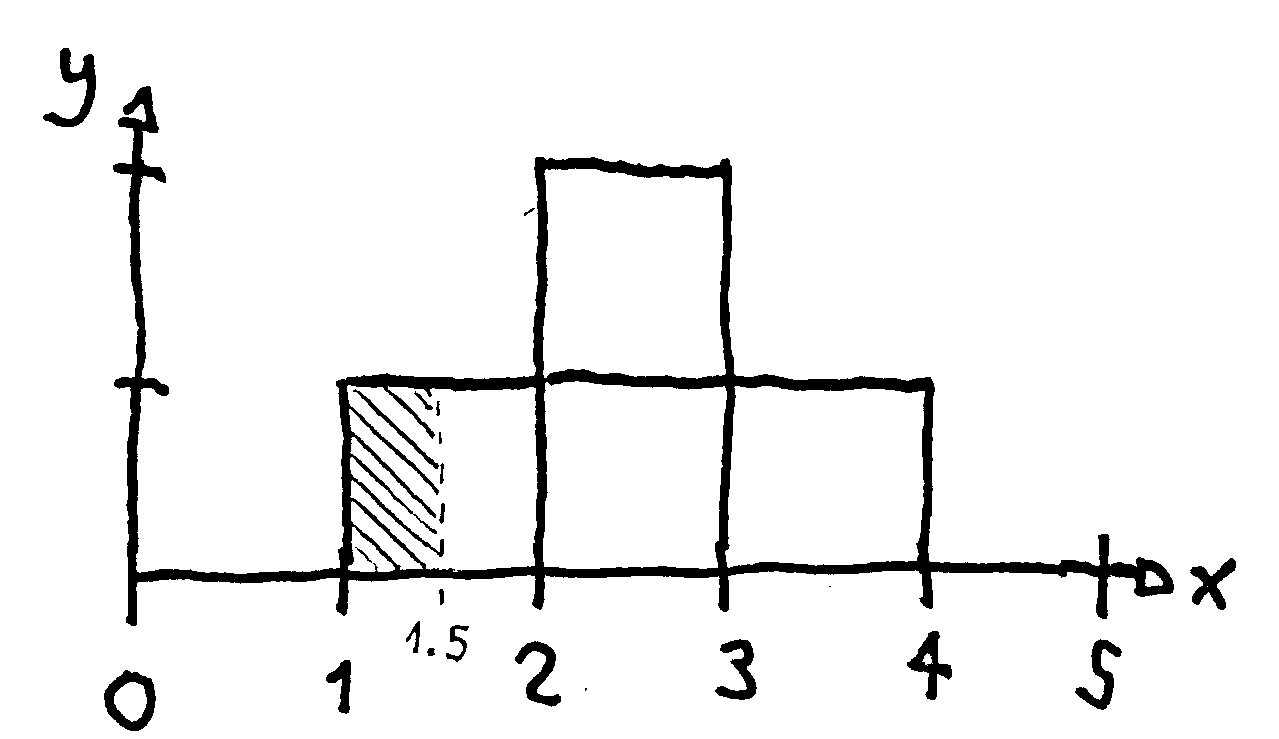
\includegraphics[height=4cm]{2023-1-ES/est-P2-fig1.pdf}$$
%
então $P(A≤1.5) = 1/8$.

\msk

a) \B(2.0 pts) Seja $B$ a distribuição contínua abaixo à esquerda.
Complete a tabela abaixo à direita. \standout{Importante:} nesta prova
você não precisa simplificar ou calcular frações -- se você chegar num
resultado como $3+\frac{2}{14}$ você pode responder $3+\frac{2}{14}$
mesmo, não precisa transformá-lo em $3.142857$.

$$
  % (find-latexscan-links "ES" "est-P2-fig2")
  % (find-xpdf-page "~/LATEX/2023-1-ES/est-P2-fig2.pdf")
  \myvcenter{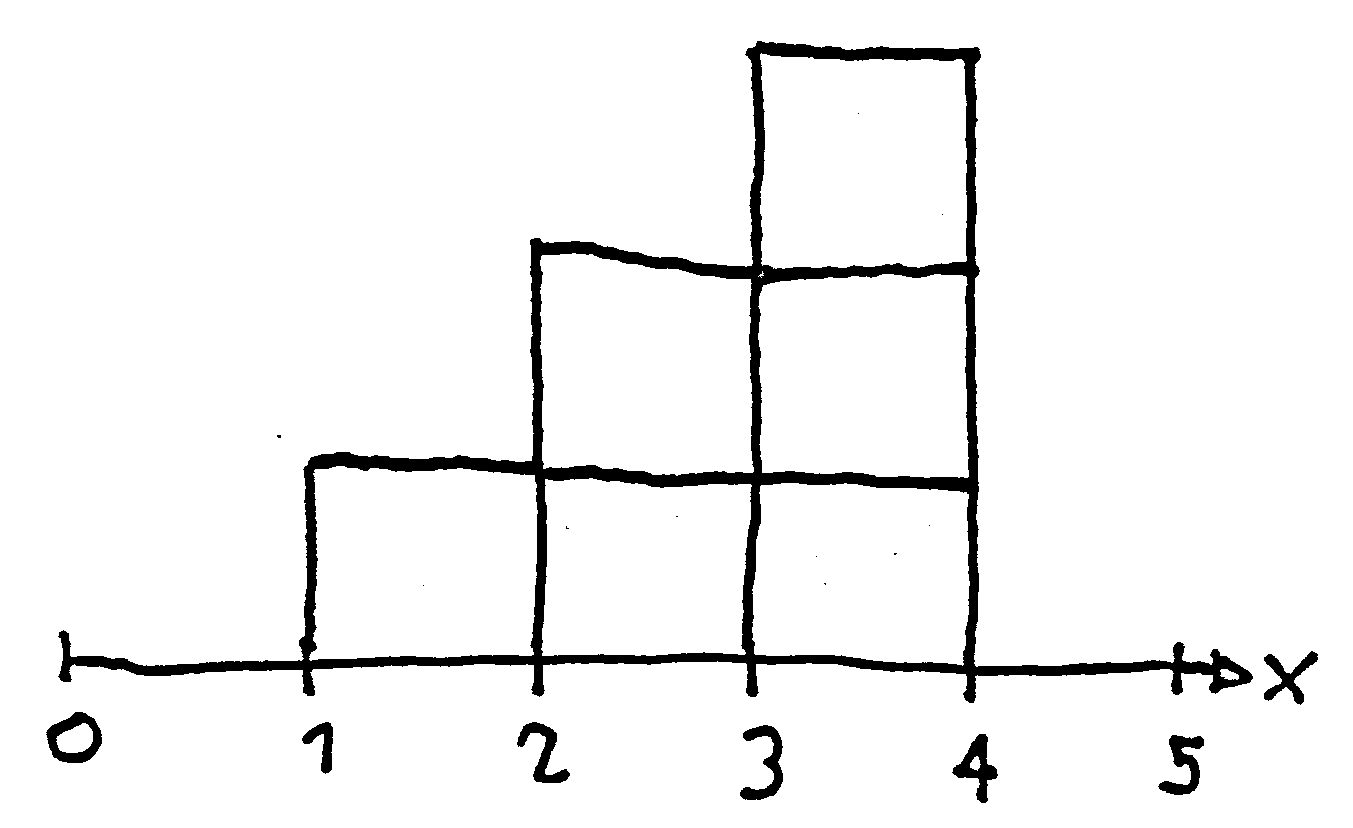
\includegraphics[width=4cm]{2023-1-ES/est-P2-fig2.pdf}}
  \quad
  \begin{array}{cl}
  x & P(B≤x) \\\hline
  0.0 \\
  0.5 \\
  1.0 \\
  1.5 \\
  2.0 \\
  2.5 \\
  3.0 \\
  3.5 \\
  4.0 \\
  \end{array}
  \qquad
$$

}\anothercol{

\vspace*{0.25cm}

No curso nós aprendemos o que são quantis usando
principalmente exemplos, porque a definição de quantil que aparece
no livro é meio complicada... por exemplo, para a variável $A$ da
figura à esquerda temos $P(A≤1.5)=1/8=12.5\%$, e portanto
$q(1/8)=q(12.5\%)=1.5$. Note que os quantis dependem da distribuição
-- o $q(1/8)$ para a variável $B$ pode ter um valor totalmente
diferente do $q(1/8)$ para a variável $A$.

\bsk

b) \B(3.0 pts) Seja $C$ esta distribuição contínua:

% (find-latexscan-links "ES" "est-P2-fig3")
% (find-xpdf-page "~/LATEX/2023-1-ES/est-P2-fig3.pdf")
$$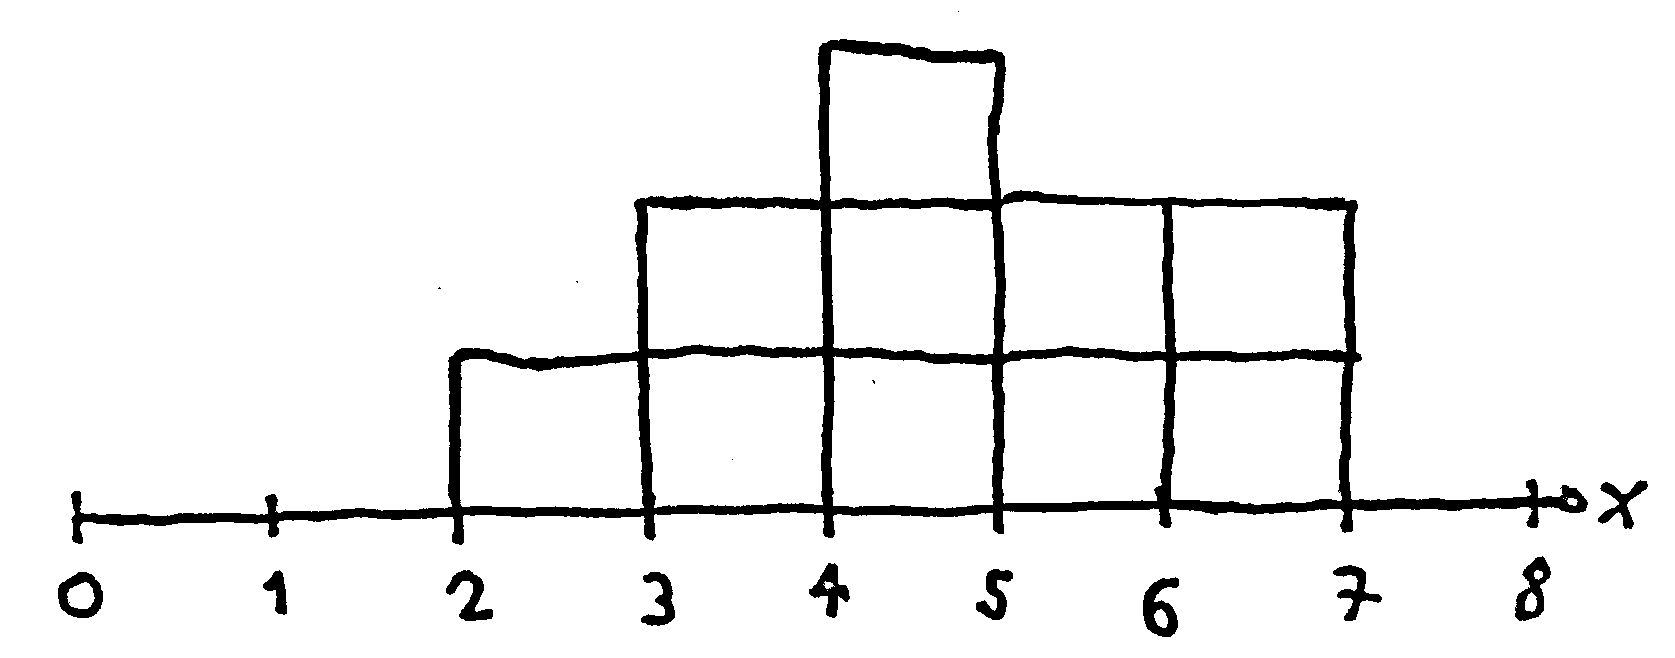
\includegraphics[width=8cm]{2023-1-ES/est-P2-fig3.pdf}$$


Complete a tabela abaixo com os quantis para a variável $C$.

$$\begin{array}{cl}
  q(10\%) = \\
  q(20\%) = \\
  q(30\%) = \\
  q(40\%) = \\
  q(50\%) = \\
  q(60\%) = \\
  q(70\%) = \\
  q(80\%) = \\
  q(90\%) = \\
  \end{array}
  \qquad
$$



}}


\newpage

%   ___                  _                ____  
%  / _ \ _   _  ___  ___| |_ __ _  ___   |___ \ 
% | | | | | | |/ _ \/ __| __/ _` |/ _ \    __) |
% | |_| | |_| |  __/\__ \ || (_| | (_) |  / __/ 
%  \__\_\\__,_|\___||___/\__\__,_|\___/  |_____|
%                                               
% «questao-2»  (to ".questao-2")
% (esm231p2p 3 "questao-2")
% (esm231p2a   "questao-2")

%L PictBounds.setbounds(v(0,0), v(6,5))
\pu

{\bf Questão 2}

\scalebox{0.6}{\def\colwidth{9cm}\firstcol{

\vspace*{-0.25cm}

\T(Total: 5.0 pts)

No curso a gente viu vários jeitos de visualizar ``váriaveis com nomes
longos''; por exemplo, no último desenho da primeira coluna da folha
de dicas da P1 -- a página 5 do PDF da prova -- eu desenhei o valor de
cada $(X-\ovl X)^2$ dentro do quadradinho correspondente.

\msk

Nesta questão você vai ter que calcular $\Cov(X,Y)$ para várias
distribuições em duas variáveis. A definição é:
%
$$\begin{array}{rcl}
  \Cov(X,Y) &=&                    \ovl{ (X-\ovl X)(Y-\ovl Y) } \\
            &=& \frac{1}{N} \sum_{i=1}^N \P{ (X_i-\ovl X)(Y_i-\ovl Y) }\\
  \end{array}
$$

Para cada uma das distribuições em duas variáveis à direita calcule
$\Cov(X,Y)$ usando as dicas que eu vou pôr no quadro (e que depois
viraram a página 4 do PDF da prova).



}\anothercol{

\vspace*{0cm}

\def\pitem#1#2{#1) \;\; \pdots{#2}}

\unitlength=10pt

$\begin{array}{rr}
 \pitem a {1,1 2,2 3,3 4,4 5,5} &
 \pitem b {2,1 3,2 4,3 5,4 6,5} \\\\[-5pt]
 \pitem c {1,3 2,2 3,1}         &
 \pitem d {1,4 2,3 3,2}         \\\\[-5pt]
 \pitem e {2,3 1,2 2,2 3,2 2,1} &
 \pitem f {1,3 3,3 2,2 1,1 3,1} \\\\[-5pt]
 \pitem g {2,3 2,2 2,1}                 &
 \pitem h {1,2 2,2 3,2}                 \\\\[-5pt]
 \pitem i {1,1 2,2 3,3 4,4 5,5 2,4 4,2} &
                                        \\
 \end{array}
$



}}

\newpage

% (find-latexscan-links "ES" "est-P2-quadro")

\vspace*{-1cm}

% (find-latexscan-links "ES" "est-P2-quadro")
% (find-xpdf-page "~/LATEX/2023-1-ES/est-P2-quadro.pdf")
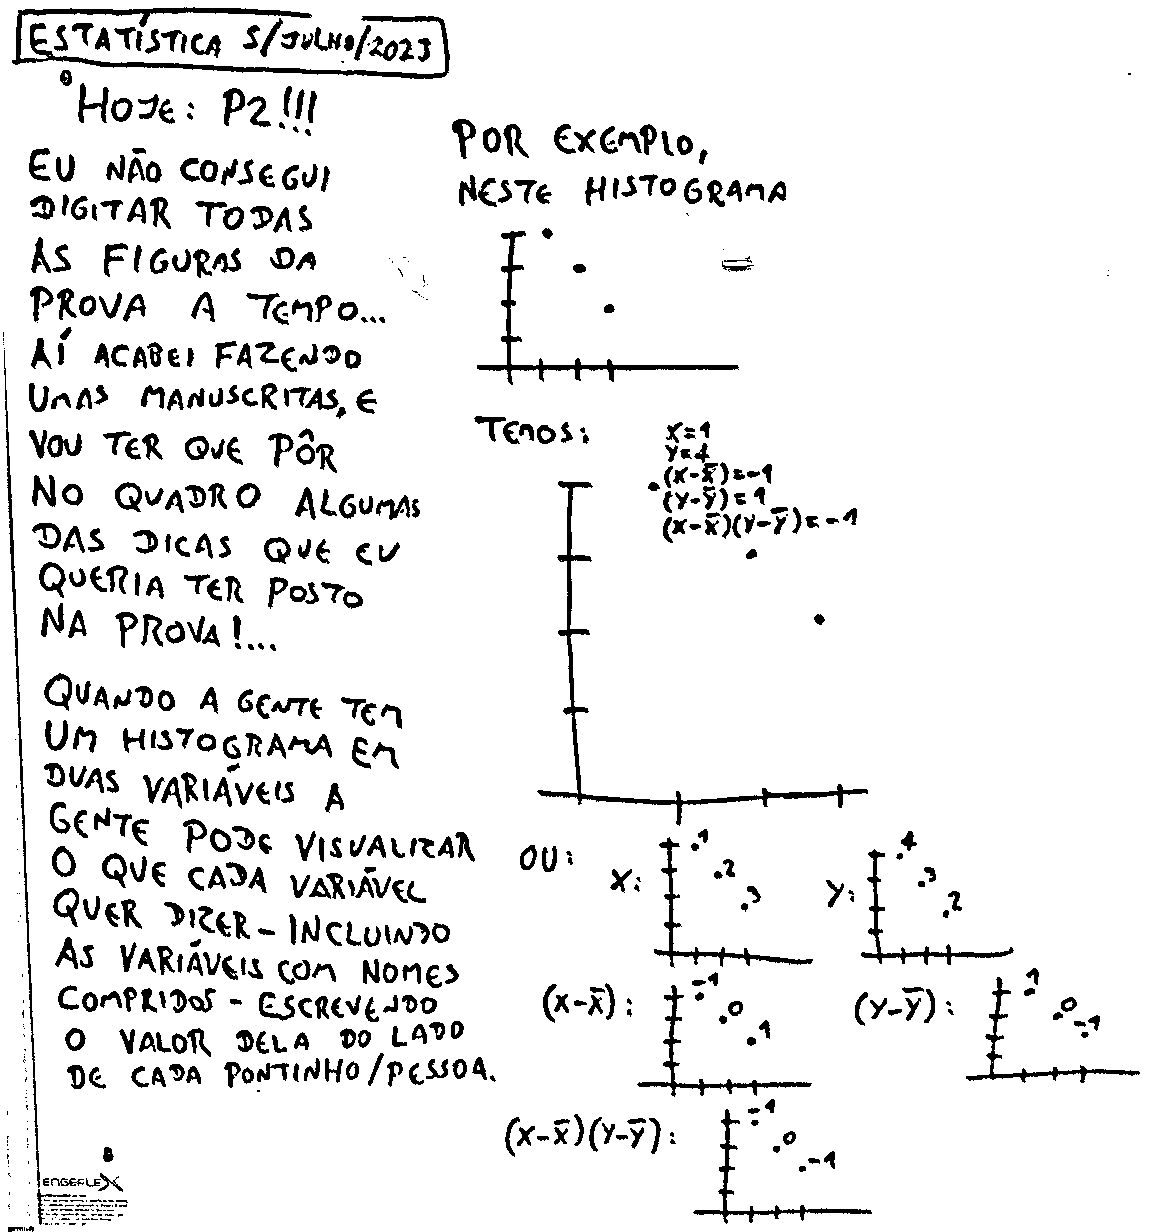
\includegraphics[height=8.5cm]{2023-1-ES/est-P2-quadro.pdf}


\newpage

%  ____  _               
% |  _ \(_) ___ __ _ ___ 
% | | | | |/ __/ _` / __|
% | |_| | | (_| (_| \__ \
% |____/|_|\___\__,_|___/
%                        

\vspace*{-0.5cm}

\scalebox{0.45}{\def\colwidth{8cm}\firstcol{

% «dicas-medias»  (to ".dicas-medias")
% (esm231p1p 4 "dicas-medias")
% (esm231p1a   "dicas-medias")

{\bf Médias}

\unitlength=13pt

\ssk

Definição: $\ovl{X} = \frac{1}{N} \sum_{i=1}^N X_i$.

\ssk

Digamos que temos duas variáveis, $A$ e $D$ -- ``antes'' e ``depois''
-- que dizem o número de paçocas de cada criança antes e depois do
Carlos dar uma paçoca pra Beatriz. As distribuições de $A$ e de $D$
são diferentes, mas como o número total de paçocas não mudou as médias
dessas duas distribuições são iguais: $\ovl{A} = \ovl{D}$. Por
exemplo:


$$\begin{array}{clccc}
  i & \nome_i & A_i & D_i \\
  \hline
  1 & \text{Ana}     & 1 & 1 \\
  2 & \text{Beatriz} & 1 & 2 \\
  3 & \text{Carlos}  & 4 & 3 \\
  4 & \text{Dani}    & 5 & 5 \\
  \end{array}
$$
$$\Media\P{\ga{pacocas 1}} =
  \Media\P{\ga{pacocas 2}}
$$

\bsk

% «dicas-dm-e-var»  (to ".dicas-dm-e-var")
% (esm231p1p 4 "dicas-dm-e-var")
% (esm231p1a   "dicas-dm-e-var")

{\bf Desvio médio e variância}

\ssk

$\DM(X)  = \frac{1}{N} \sum_{i=1}^N |X_i - \ovl{X}|$

$\Var(X) = \frac{1}{N} \sum_{i=1}^N (X_i - \ovl{X})^2$

\ssk

Lembre que $|42|=42$, $|-42|=42$, e que nas aulas a gente calculou o
desvio médio e a variância usando ``histogramas com numerozinhos'',
como esses aqui:
%
$$\scalebox{1.5}{$
  \ga{dm} \qquad \ga{var}
  $}
$$


}\anothercol{

% «dicas-probabilidade»  (to ".dicas-probabilidade")
% (esm231p1p 4 "dicas-probabilidade")
% (esm231p1a   "dicas-probabilidade")

{\bf Probabilidade}

Uma variável que só pode assumir os valores `$\True$' (verdadeiro) ou
`$\False$' (falso) é uma variável {\sl booleana}.

A operação $[·]$ (``colchete'') transforma boole\-anos nos valores 0 e
1. Por exemplo:
%
$$\begin{array}{c}
  [2<3] = [\True] = 1,   \\{}
  [2>3] = [\False] = 0.  \\
  \end{array}
$$
%
Se $B$ é uma variável booleana e todas as linhas da nossa tabela são
``equiprováveis'' então a probabilidade de $B$, $P(B)$ é definida
assim:
%
$$P(B) = \frac{1}{N} \sum_{i=1}^N [B_i].$$
%
Às vezes a gente intepreta expressões como `$A<42$' como {\sl
  variáveis com nomes longos} -- e aí $(A<42)_i = (A_i<42)$. E às
vezes a gente coloca definições na primeira linha da tabela. Por
exemplo, em
%
$$\begin{array}{cccc}
  i & A_i & B_i=(A_i<42) & C_i=[B_i] \\
  \hline
  1 & 200 & \False & 0 \\
  2 & 20  & \True  & 1 \\
  3 & 99  & \False & 0 \\
  \end{array}
$$
%
a segunda coluna diz que cada $B_i$ vai ser definido como o resultado
do $A_i<42$ correspondente e lista os valores dos `$B_i$'s, e a
terceira coluna faz a mesma coisa pros `$C_i$'s.

Neste caso temos $\ovl{C} = \ovl{[B]} = \frac13$ e:
%
$$P(B) = P(A<42) = \frac13.$$


}\anothercol{

% «dicas-conjuntos»  (to ".dicas-conjuntos")
% (esm231p1p 4 "dicas-conjuntos")
% (esm231p1a   "dicas-conjuntos")

\sa {A}          {\unddots{A}{1,2 2,2}}
\sa       {B}    {\unddots{B}{2,2 2,1}}
\sa {A cap B}    {\unddots{\ga{A}∩\ga{B}}{2,2}}
\sa{(A cap B)^c} {\unddots{(\ga{A cap B})^c}{2,1 1,1 1,2}}
\sa{A^c}         {\unddots{(\ga{A})^c}{1,1 2,1}}
\sa        {B^c} {\unddots{(\ga{B})^c}{1,1 1,2}}
\sa{A^c cup B^c} {\unddots{\ga{A^c}∪\ga{B^c}}{2,1 1,1 1,2}}

{\bf Conjuntos}  

\ssk

\unitlength=4pt

Se $Ω=\{1,2,3,4\}$, $A=\{1,2\}$ e $B=\{2,3\}$

então $A∪B = \{1,2,3\}$, $A∩B=\{2\},$

e $A^c = \{3,4\}$.

\ssk

%L PictBounds.setbounds(v(0,0), v(2,2))
\pu

\unitlength=6pt

Se $Ω = \pdots{1,1 1,2 2,1 2,2}$,
   $A = \pdots{    1,2     2,2}$ e
   $B = \pdots{        2,1 2,2}$,
   então:

\unitlength=4pt

$$%
  \und{
    \ga{(A cap B)^c} \;=\;
    \ga{A^c cup B^c}
  }{\True}
$$

\msk

Às vezes a gente diz qual é a probabilidade de cada ``evento''. Nós
usamos este exemplo aqui várias vezes:

\unitlength=6pt

$$\def\PP#1#2{P \P{\pdots{#1}}=\frac{#2}{10}}
  \begin{array}{c}
  \PP{1,2}{1}, \; \PP{2,2}{2}, \\
  \PP{1,1}{3}, \; \PP{2,1}{4}.
  \end{array}
$$

Quando a gente não diz a probabilidade de cada evento fica implícito
que eles são equiprováveis.

\bsk
\bsk

% «dicas-prob-cond»  (to ".dicas-prob-cond")
% (esm231p1p 4 "dicas-prob-cond")
% (esm231p1a   "dicas-prob-cond")

{\bf Probabilidade condicional}

A definição é: $P(A|B) = P(A∩B) / P(B)$.

%L PictBounds.setbounds(v(0,0), v(3,3))
\pu
\unitlength=6pt

Por exemplo:

$P\P{\pdots{1,3 2,2 3,1} \;\; | \;\;
     \pdots{2,3 3,3 2,2 3,2 2,1 3,1}}
 =
 P\P{\pdots{    2,2 3,1}} /
 P\P{\pdots{2,3 3,3 2,2 3,2 2,1 3,1}}.
$

}}





% (find-latexscan-links "ES" "est-P2-fig3")
% (find-xpdf-page "~/LATEX/2023-1-ES/est-P2-fig3.pdf")
%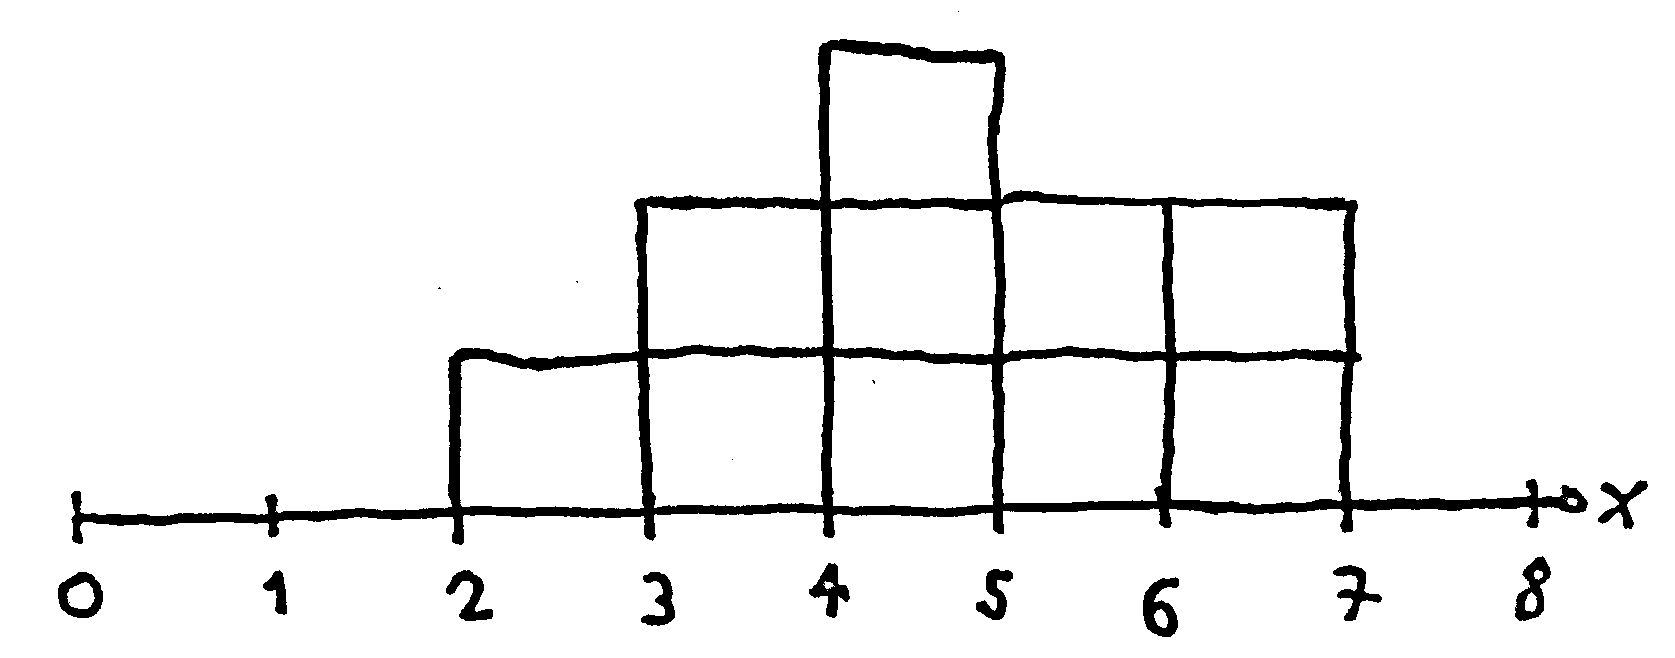
\includegraphics[height=8cm]{2023-1-ES/est-P2-fig3.pdf}





%L Pict.__index.enslower = -0.25
%L Pict.__index.enslower = -0.4
%L
%L -- Exemplo das paçocas:
%L PictBounds.setbounds(v(0,0), v(6,2))
%L spec1 = "1:A 1:B 4:C 5:D"
%L spec2 = "1:A 2:B 3:C 5:D"
%L p1    = SqP.from(spec1):topict():scalebox(0.6):sa("pacocas 1")
%L p2    = SqP.from(spec2):topict():scalebox(0.6):sa("pacocas 2")
%L Pict { p1, p2 } :output()
%L
%L -- Histogramas com numerozinhos pra desvio médio e variância:
%L PictBounds.setbounds(v(0,0), v(6,1))
%L specdm  = "1:2 2:1 3:0 4:1 5:2"
%L specvar = "1:4 2:1 3:0 4:1 5:4"
%L p1      = SqP.from(specdm ):topict():scalebox(0.6):sa("dm")
%L p2      = SqP.from(specvar):topict():scalebox(0.6):sa("var")
%L Pict { p1, p2 } :output()
\pu

%$\ga{pacocas 1}
% \ga{pacocas 2}
% \ga{dm}
% \ga{var}
%$



\newpage

% «links»  (to ".links")

\GenericWarning{Success:}{Success!!!}  % Used by `M-x cv'

\end{document}

%  ____  _             _         
% |  _ \(_)_   ___   _(_)_______ 
% | | | | \ \ / / | | | |_  / _ \
% | |_| | |\ V /| |_| | |/ /  __/
% |____// | \_/  \__,_|_/___\___|
%     |__/                       
%
% «djvuize»  (to ".djvuize")
% (find-LATEXgrep "grep --color -nH --null -e djvuize 2020-1*.tex")

 (eepitch-shell)
 (eepitch-kill)
 (eepitch-shell)
# (find-fline "~/2023.1-ES/")
# (find-fline "~/LATEX/2023-1-ES/")
# (find-fline "~/bin/djvuize")

cd /tmp/
for i in *.jpg; do echo f $(basename $i .jpg); done

f () { rm -v $1.pdf;  textcleaner -f 50 -o  5 $1.jpg $1.png; djvuize $1.pdf; xpdf $1.pdf }
f () { rm -v $1.pdf;  textcleaner -f 50 -o 10 $1.jpg $1.png; djvuize $1.pdf; xpdf $1.pdf }
f () { rm -v $1.pdf;  textcleaner -f 50 -o 20 $1.jpg $1.png; djvuize $1.pdf; xpdf $1.pdf }

f () { rm -fv $1.png $1.pdf; djvuize $1.pdf }
f () { rm -fv $1.png $1.pdf; djvuize WHITEBOARDOPTS="-m 1.0 -f 15" $1.pdf; xpdf $1.pdf }
f () { rm -fv $1.png $1.pdf; djvuize WHITEBOARDOPTS="-m 1.0 -f 30" $1.pdf; xpdf $1.pdf }
f () { rm -fv $1.png $1.pdf; djvuize WHITEBOARDOPTS="-m 1.0 -f 45" $1.pdf; xpdf $1.pdf }
f () { rm -fv $1.png $1.pdf; djvuize WHITEBOARDOPTS="-m 0.5" $1.pdf; xpdf $1.pdf }
f () { rm -fv $1.png $1.pdf; djvuize WHITEBOARDOPTS="-m 0.25" $1.pdf; xpdf $1.pdf }
f () { cp -fv $1.png $1.pdf       ~/2023.1-ES/
       cp -fv        $1.pdf ~/LATEX/2023-1-ES/
       cat <<%%%
% (find-latexscan-links "ES" "$1")
%%%
}

f est-P2-fig1
f est-P2-fig2
f est-P2-fig3
f est-P2-quadro

f 20201213_area_em_funcao_de_theta
f 20201213_area_em_funcao_de_x
f 20201213_area_fatias_pizza



%  __  __       _        
% |  \/  | __ _| | _____ 
% | |\/| |/ _` | |/ / _ \
% | |  | | (_| |   <  __/
% |_|  |_|\__,_|_|\_\___|
%                        
% <make>

 (eepitch-shell)
 (eepitch-kill)
 (eepitch-shell)
# (find-LATEXfile "2019planar-has-1.mk")
make -f 2019.mk STEM=2023-1-ES-P2 veryclean
make -f 2019.mk STEM=2023-1-ES-P2 pdf

% Local Variables:
% coding: utf-8-unix
% ee-tla: "esp2"
% ee-tla: "esm231p2"
% End:
